\documentclass[11pt]{article}  % [12pt] option for the benefit of aging markers
\usepackage{amssymb,amsthm}    % amssymb package contains more mathematical symbols
\usepackage{graphicx}          % graphicx package enables you to paste in graphics
\usepackage[document]{ragged2e} 
\usepackage{float}
\usepackage{tabularx}
\usepackage{multirow}
\usepackage{setspace}
\usepackage{adjustbox}

%%%%%%%%%%%%%%%%%%%%%%%%%%%%%%%%%
%
%    Page size commands.  Don't worry about these
%
\setlength\topmargin{0pt}
\addtolength\topmargin{-\headheight}
\addtolength\topmargin{-\headsep}
\setlength\oddsidemargin{0pt}
\setlength\textwidth{\paperwidth}
\addtolength\textwidth{-2in}
\setlength\textheight{\paperheight}
\addtolength\textheight{-2in}
\doublespacing

%%%%%%%%%%%%%%%%%%%%%%%%%%%%%%%%%%%%%%%%%%%%%%%%%%%%%%%%%%%%%%%
%
%    Definitions of environments for theorems etc.
%
\newtheorem{theorem}{Theorem}[section]          % Theorems numbered within sections - eg Theorem 2.1 in Section 2.
\newtheorem{corollary}[theorem]{Corollary}      % Corollaries etc. will be counted as Theorems for numbering
\newtheorem{lemma}[theorem]{Lemma}              % eg Lemma 3.1, ... Theorem 3.2, ... Corollary 3.3.
\newtheorem{proposition}[theorem]{Proposition}
\newtheorem{conjecture}[theorem]{Conjecture}

\theoremstyle{definition}
\newtheorem{definition}[theorem]{Definition}

\theoremstyle{remark}
\newtheorem{remark}[theorem]{Remark}
\newtheorem{example}[theorem]{Example} 
\graphicspath{ {./Images/} }

%%%%%%%%%%%%%%%%%%%%%%%%%%%%%%%%%%%%%%%%%%%%%%%
%
%        Preamble material specific to your essay
%
\title{Evaluation of Mastermind Solutions\\
Deliverable 1: Research Report}
\author{Kyle Dick\\
F20PA Project\\
supervised by
Kathrin Stark}

\begin{document}
\maketitle

\newpage                     % optional page break
\begin{abstract}

Mastermind is a two-player game which tasks player A with breaking a code created by player B. The code breaking process consists of making queries regarding the shape of the secret code which is rewarded with hints as to the accuracy of these queries. Beneath this simple game concept lies a complex combinatorial search problem focused on selecting a correct code combination from the set of all possible code combinations constructed from a set of symbols. Investigation into a variety of search algorithms which employ both exhaustive, non-exhaustive and evolutionary strategies aims to further understand how these search algorithms can be adapted to fit larger search spaces.


\end{abstract}

\newpage                     % optional page break
\tableofcontents

\newpage                     % optional page break
\section{Introduction}\label{s:intro}
%
%In recent times a global interest has developed around the linguistic game Wordle. The concept of this puzzle is simple, the user is to 
%guess a five letter word in as few guesses as possible within six attempts. After each guess the computer will inform the user if a letter 
%was in the correct position, denoted as a green highlight, or is contained within the word but not in the correct position, denoted with a yellow highlight.
\justify{
Mastermind is a two-player coded-breaking game in which one player is tasked with discovering a secret combination set by the other player.
The puzzle is a member of problems known as combinatorial problems where the goal is to find the correct combination of elements from a finite
set to satisfy a given set of conditions. The process of investigating possible solutions to the Mastermind puzzle has been underway for decades
however there exists some difficulties in defining a clear solution to this day. The implementation of a solution to the Mastermind puzzle would provide
benefits to several problems faced in many sectors of the real world such as cyber security which retains the solutions value as a goal worth seeking.
Currently the challenges that are being faced in this endeavour relate to finding methods of determining the correct decisions to be made when formulating
guesses at each step of the puzzle. Several attempts at defining a solution have yielded promising results yet a common occurrence is that these
implementations struggle when attempting to address variations of the standard Mastermind puzzle.

The implementation that this project seeks to develop will use the foundations provided by the advancements made until the present day. An implementation
based in the field of functional programming was chosen as the ideal candidate as among other factors which will be discussed further in later sections,
functional programming provides mitigation against variance in outputs which would contribute to confusion when seeking a rigid solution.}

\subsection {Aims and Objectives}
The aims and objectives of this project can be surmised in two specific goals. The first goal is to derive a solution to the logical puzzle 
Mastermind. The second goal is to evaluate solutions implemented during this project with the aim to find methods to improve later 
iterations. An in depth explanation of the chosen aims and objectives are as such:

\

\textbullet\ Aim 1: To derive a solution to the puzzle Mastermind.

\

The goal to find a solution to the problem which minimises the number of guesses required to discover the correct combination of
pegs which comprise the code. Initially the goal will be to derive a base solution to the Mastermind puzzle. The base solution being the
most intuitive solution to the problem which does not aim to be the most efficient but to provide a foundation on which improvements
can be made. The following objectives are associated with this aim:

\

\textbullet\ Objective 1.A: Investigate the problem space.

\

The Mastermind puzzle has previously been the subject of similar research regarding the ability to efficiently find the correct code
combination. This stage of the project will concern itself with investigating these previous implementations to guide the project.
Through exploring the methods utilised in other investigations into this problem the areas in which these solutions are lacking or could
improvements can be found. The research presented in this report represents the progress of this objective.

\

\textbullet\ Objective 1.B:  Implement a base solution.

\

The ideal base solution should achieve the basic goal of arriving at the correct code combination but should not be the most elegant
solution at this point. Instead the base solution should be the foundation for which improvements are made in later iterations.
The base solution will be guided through the research conducted through objective 1.A.

\

\textbullet\ Aim 2: Optimise the Mastermind Solution.

\

The next step following the creation of a base solution is the optimization of this implementation. The goal with optimization is to discover
new methods of how the solution can be improved in regards to its efficiency. In the context of the Mastermind puzzle the concept of a
search space is an important factor to optimization as it refers to the set of possible codes which satisfy the problem. An example of how
the solution could be optimised is by considering ways in which this search space could be either minimised or how the navigation of the
space can be improved.


\

\textbullet\ Objective 2.A: Explore Methods of Optimising the Search Space.

\

The optimization of the problem's search space is directly linked to the measure of efficiency when considering Mastermind solutions.
An of how this can be achieved is by implementing methods of minimising the search space such that the quantity of possible codes
which could satisfy the problem. The other method that should be investigated is improvements to how the search space
is navigated by the solution. This is a method which relates heavily to the concept of heuristics and assigning values to the items within
the search space which will be covered in a later section of this report. These are not the only methods that exist to optimise the
search space and the exploration of differing methods is to be encouraged and sought out should it be possible.

\

\textbullet\ Objective 2.B: Explore Methods of Measuring the Efficiency of a Solution.

\

To achieve the goal of optimising the solution it is important to define the elements which are being optimised for. An example of
This is already defined by the previous objective in regards to search space however this is not the only area which can be optimised.
The question that is to be answered by this objective is how other factors such as the speed at which a solution can reach a code
which satisfies the problem should be considered.


\

\textbullet\ Objective 2.C: Improve the Solution.

\

This is a continual objective which encapsulates the main goal of this aim. Measurements of the optimization as defined by previous 
objectives should reflect the improvements made in later iterations of the solution. Documentation of the results of each optimization 
method should be presented as a component of this objective.

\

\textbullet\ Aim 4: Investigate Solutions to Mastermind Variants.

\

A topic that is a recurring source of intrigue with similar research into the Mastermind puzzle is the potential for a solution to scale with
changes in the way that the code is constructed. One such change relates to the possible set of symbols which the code could contain.
This objective should consider methods of how the solution can adapt when the number of possible symbols increases above the standard six.


\

\textbullet\ Objective 4.A: Investigate Solution with Variance in Set Size for Possible Symbols.

\

A topic that is a recurring source of intrigue with similar research into the Mastermind puzzle is the potential for a solution to scale with
changes in the way that the code is constructed. One such change relates to the possible set of symbols which the code could contain.
This objective should consider methods of how the solution can adapt when the number of possible symbols increases above the standard six.

\

\textbullet\ Objective 4.B: Investigate Solution with Variance in Code Length.

\

An additional scaling factor which is an area of possible investigation is changes in the length of the code. 
The considerations regarding this objective relate to the ways in how a solution will handle the larger search space and the changes in optimization.

\

\textbullet\ Objective 4.C: Investigate Solutions to Similar Problems.

\

The solution implemented in this project could have applications beyond the initial  Mastermind puzzle. 
This objective is concerned with how the solution can be applied to other similar problems, an example of such a puzzle would be the popular language game Wordle \cite{Wordle}.

%
% The \label command is optional, but useful.  To cross-refer to a section/theorem/equation etc.
% labelled by \label{key}, use \ref{key}.  For example: Equation (\ref{eq:key}) follows from Theorem \ref{th:key}.

\newpage                     % optional page break
\section{Background}\label{ss:back}

% Summary of the background material and introduction to the section
The Mastermind puzzle has been subject to investigations regarding solutions to the code-breaking aspect of the game
since its release.
This section will provide background material which aims to give context to the aims and objectives of this project.
The project was inspired by a paper exploring sudoku solutions from a series of problems known as functional pearls,
The processes used to derive those solutions will be used to guide this project in this current stage.
Following this brief introduction is an explanation of the game Mastermind which the solution will be derived from along
with references to previous work by others. The previous work examined will focus on the specific area of search spaces
in regards to finding the optimal best move at each position in the puzzle. At the conclusion of this section the goal is
that the reader has an understanding of the important concepts relating to this project such that the aims and objectives
are clear in their feasibility and relevancy.


%%% What is the problem?
% What is the goal of Mastermind that our solution will be modelled on?
\subsection {The Mastermind Puzzle}

% A brief history and explanation of the game
Mastermind is a two-player game in which one player seeks to break a secret code combination created by the other player \cite{Wolfram}. Originally a physical board game designed by an Isreali Postmaster named Mordecai Meirowitz, distributed through Invicta Toys and Games \cite{Invicta}. Mastermind was originally designed as a two player game but it can also be treated as a puzzle due to the passive nature of the player who would create the code combination \cite {Better Solutions}. When viewed from this approach Mastermind can be explored as a puzzle which focuses on different strategies of arriving at the secret code combination, preferably in as few guesses possible.

\subsubsection {The Rules of Mastermind}

% Explanation of Mastermind puzzle
The standard variant of the puzzle as introduced in the physical board game used plastic pegs to represent both the secret combination and the attempted guesses \cite {Invicta}.
The length of a code combination in the standard variant is exactly four and can be constructed from a set of six unique colours, with duplicates permitted \cite{Wolfram}.

\begin{figure}[H]
\centering
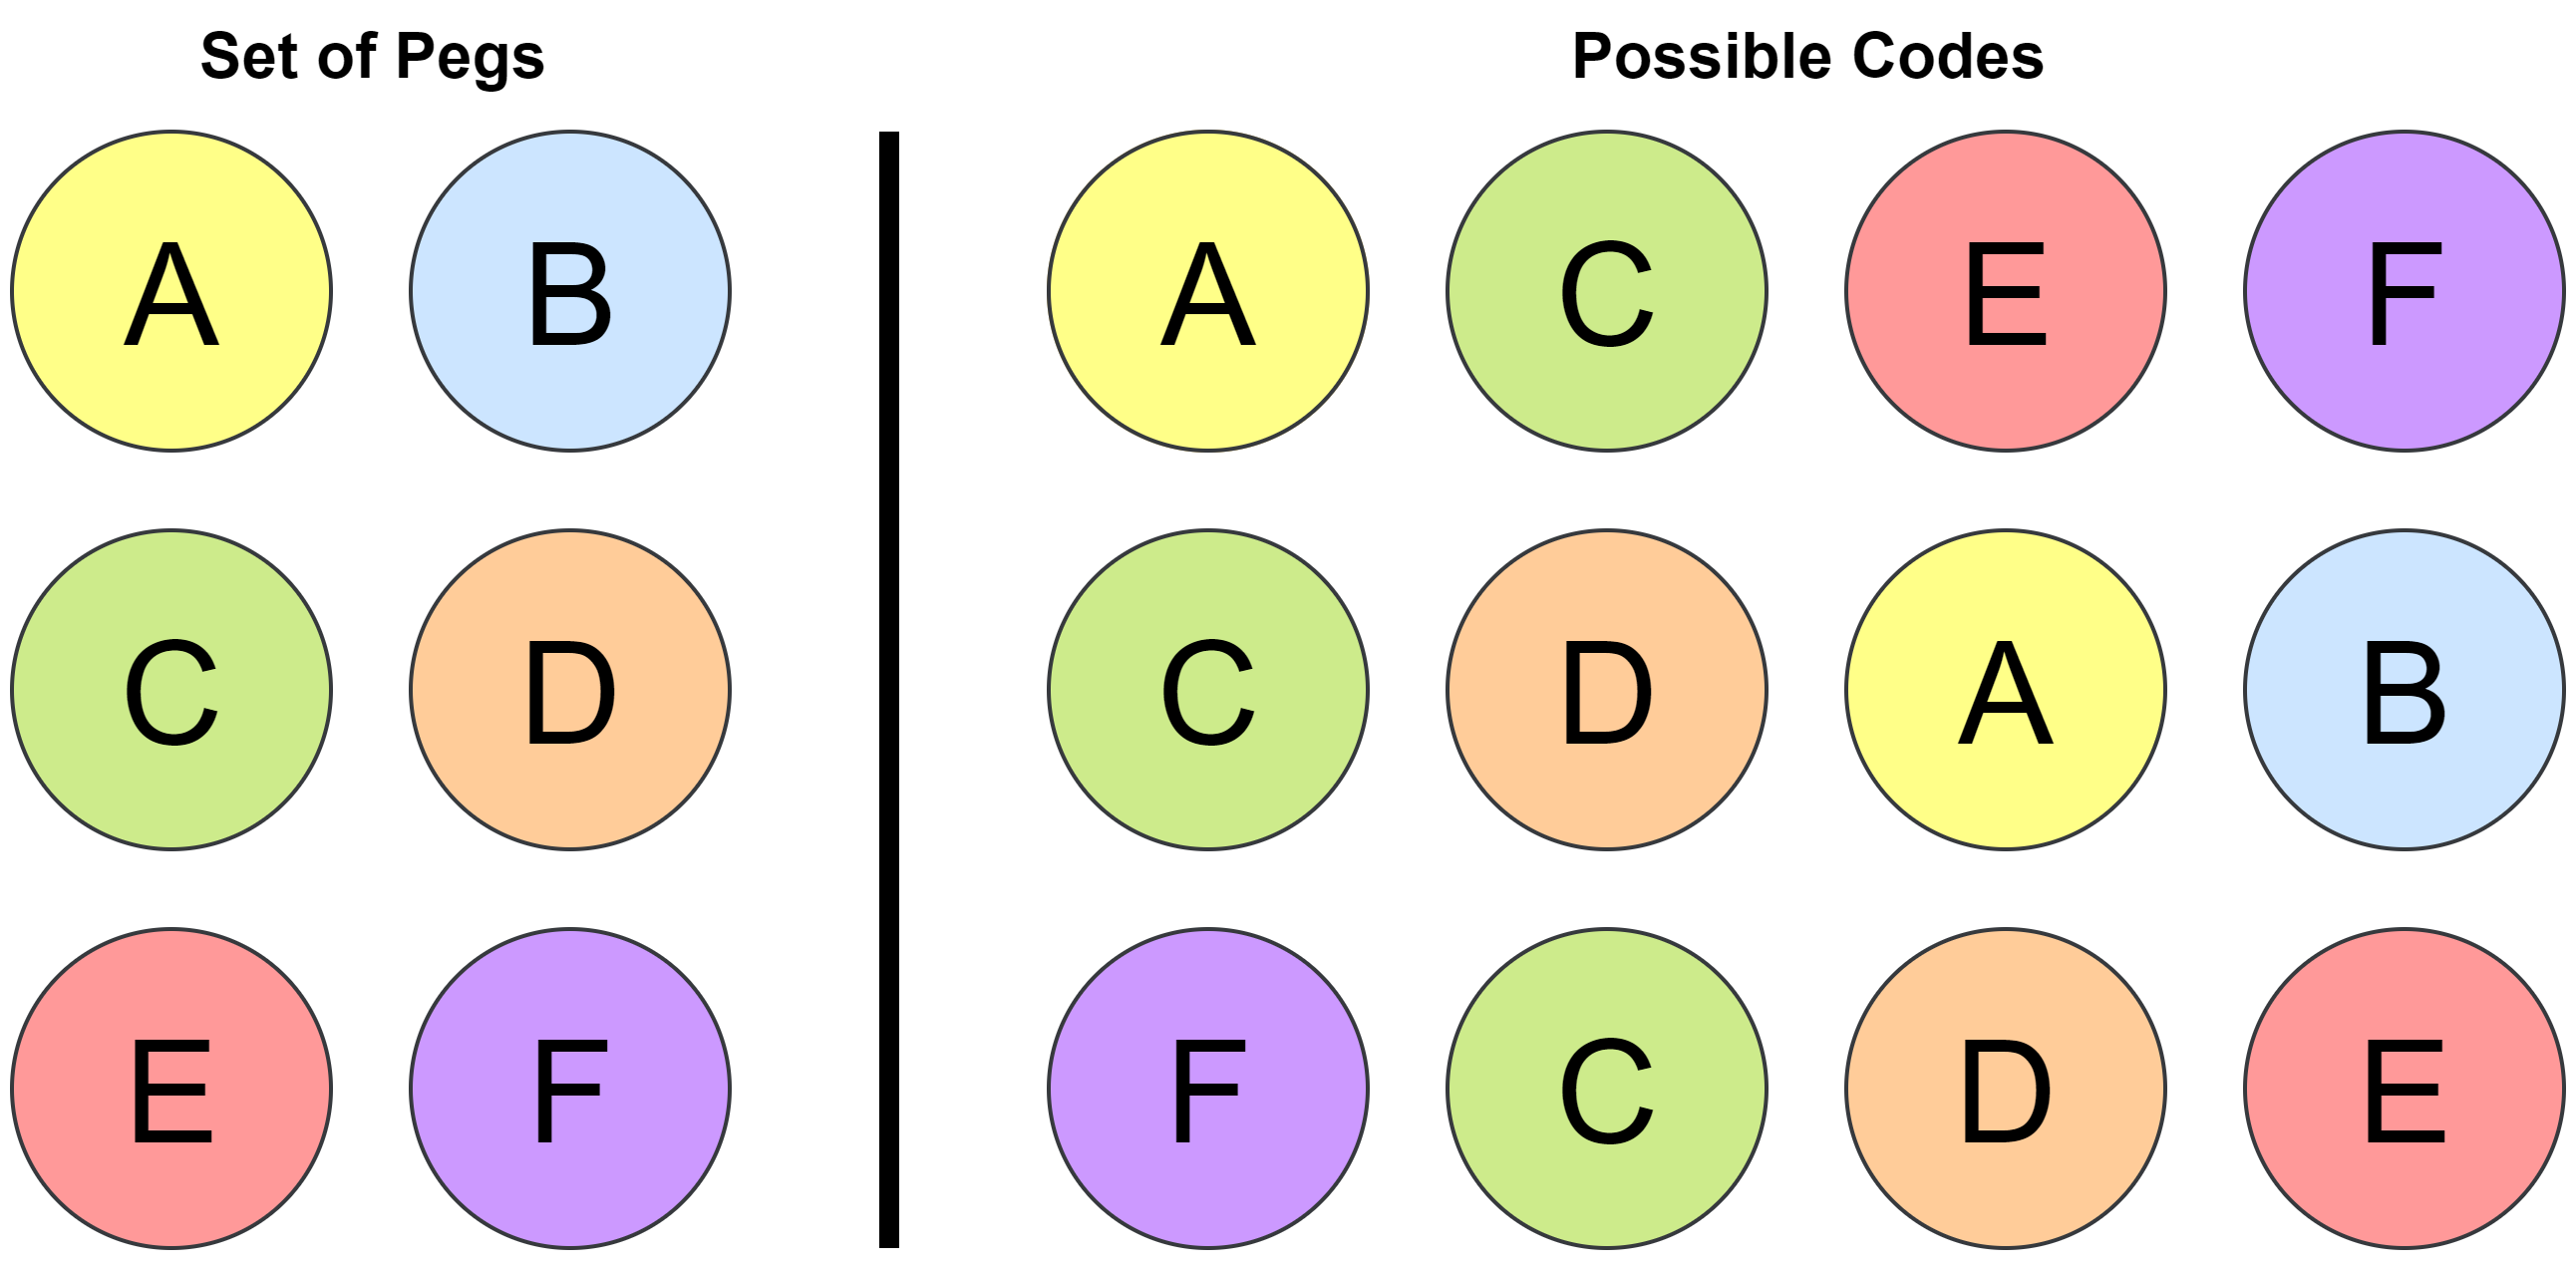
\includegraphics[scale=0.4]{pegs}
\caption{ Example codes which would satisfy the constraints of the standard variant of Mastermind.}
\end{figure}

The game begins once the secret code combination has been selected. The process of breaking the secret code consists of one player attempting a sequence of guesses as to the position and colours of the pegs in the code. Each attempt is followed by a hint which informs the player of how accurate their guess was in relation to the secret code. These hints inform the player if a correct colour was played in an incorrect position, most commonly represented with a white peg, and if a correct colour was played in a correct position, represented with a black peg.

\begin{figure}[H]
\centering
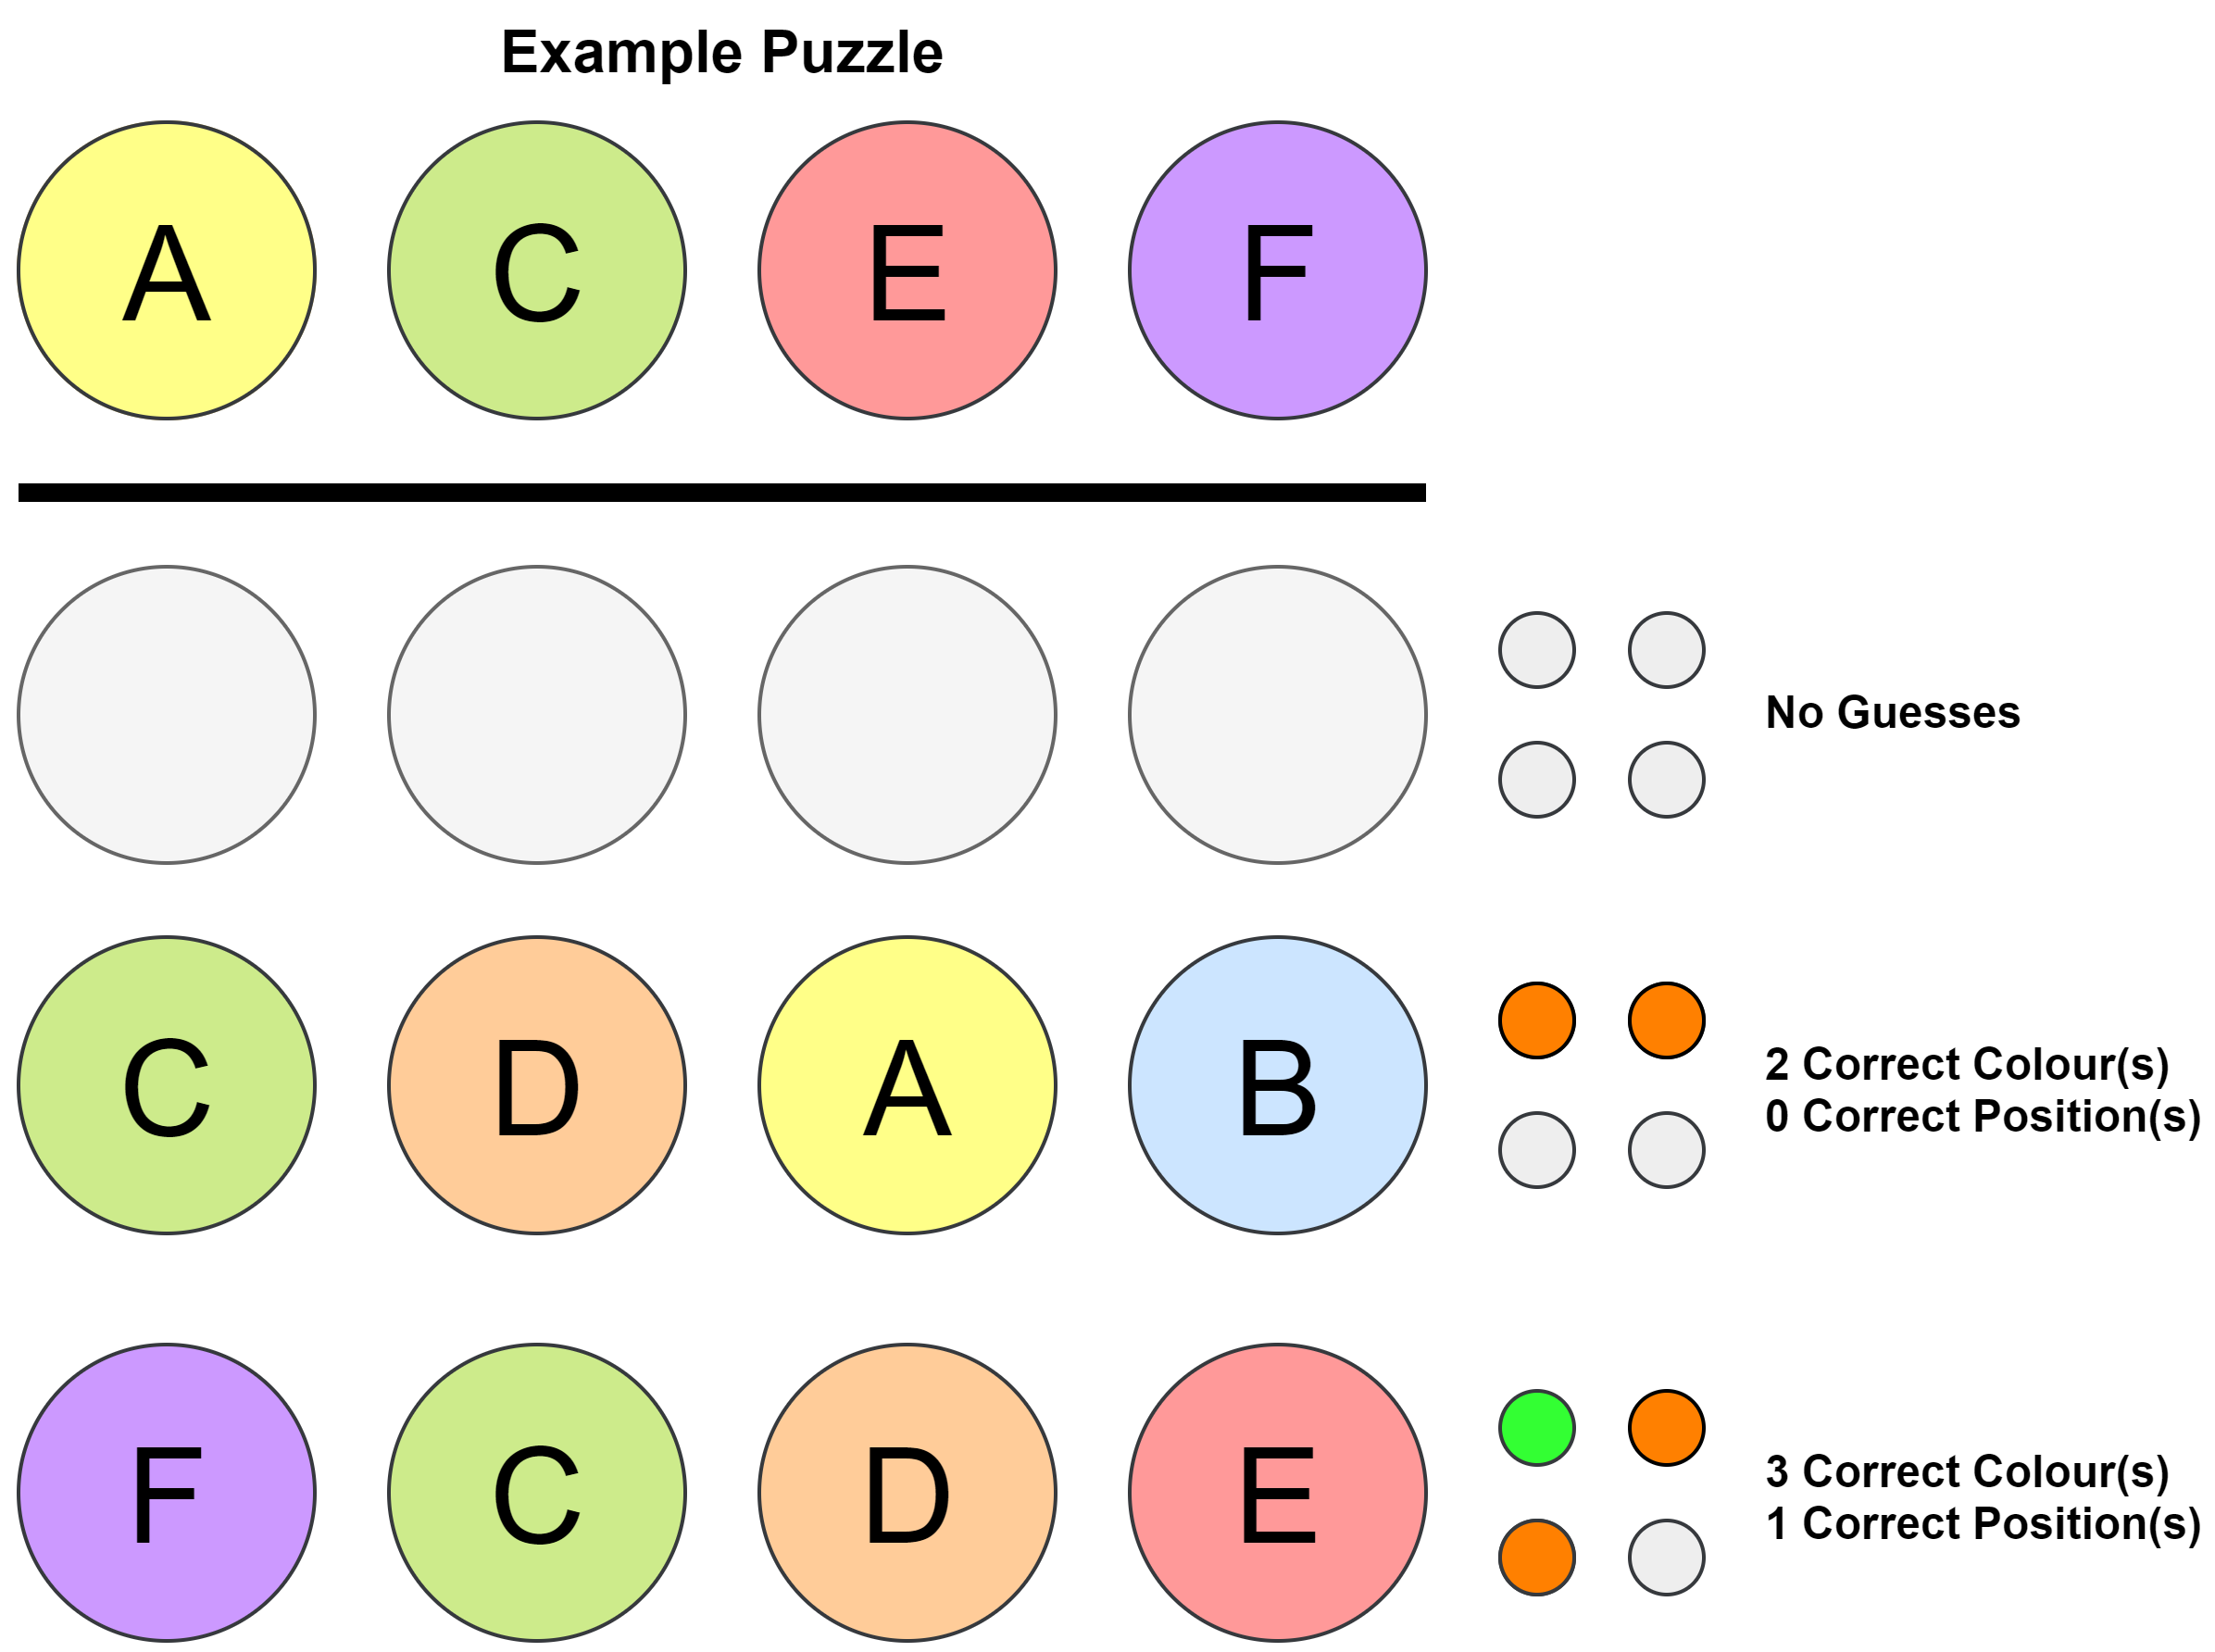
\includegraphics[scale=0.4]{guesses}
\caption{A simplified representation of a game state. The black and white hint pegs were replaced with green and amber for clarity.}
\end{figure}

The game concludes when the correct code combination is discovered, represented through the hint system as four black pegs, or if a limit of guesses would be exceeded.

\subsubsection {Variations and Similar Problems}

Multiple variations of the original Mastermind game exist, most commonly varying either the length of the secret code, the size of the set of elements a code can be constructed from or both. One such example of this is the Super Mastermind variant which increments the code length to five elements and increases the possible elements to eight \cite {SuperMM}. These alterations result in 32 768 possible code combinations which could be selected as the secret code, a substantial increase over the 1 296 combinations of the standard variant. This increase becomes relevant when attempting to implement solutions to the puzzle as searching for a correct code combination in the larger sets poses challenges in time and memory \cite {ExhaustiveMM}.

\subsection {Problem Description and Fundamental Concepts}

\subsubsection {The Goal of a Solution}
To the perspective of the codebreaker Mastermind presents itself as a search problem which examines a set of all possible combinations which satisfy the given constraints and tasks the player with identifying the secret code within the set. An effective solution to Mastermind would be one that is able to traverse this set of all possible combinations and identify the secret code combination within it.

\subsubsection {Consistency and Search Strategies}

The search space associated with the standard variant of Mastermind contains 1,296 members, a naive strategy for finding the correct code amongst the collection could evaluate each entry individually to find a match to the secret code. A strategy which can prove efficient for smaller search spaces but is not viable as the size of the collection increases \cite{Two Peg}.

Previous Mastermind solutions would introduce a concept which would allow for easier traversal of these larger search spaces in the form of consistency. The logic behind this concept is that when an attempt is made to find the secret code combination the remaining search space that needs to be evaluated in later attempts is reduced due to that combination no longer being relevant to search and the hint provided from the attempt can deduce which combinations are incompatible with the secret code \cite {Merelo}. The consideration of a combination attempt and the resulting hint can be defined as a rule for that instance \cite {Haystack}. This can be shown for the example below:

\

Consider the secret code combination which represents the characters of the code as integers: '1111'. Prior to any search attempt the full range of 1,296 code combinations are equally probable to be the secret code. An attempt to evaluate the code '2332' returns a hint of zero white pegs and zero black pegs, informing the codebreaker that the symbols '2' and '3' do not appear in the secret code and therefore are not consistent with this instance. The only remaining possible code combinations are required to be consistent with this information, this forms the consistent search space. The consistent search space for this example would include all possible code combinations excluding those which contain either symbol '2' or '3'.

The concept of a consistent search space provides the basis for two categories of Mastermind solutions \cite{Haystack}:

\textbullet\ Stepwise Optimal: This strategy only selects code combinations which are consistent with the past attempts as defined previously. This method results in less combinations requiring evaluation due to redundant examples being ignored.

\textbullet\ Strategically Optimal: This strategy selects code combinations which allow for information relating to the appearance of the secret code to be deduced. The aim of a strategically optimal search strategy is to reduce the consistent search space by attempting suboptimal code combinations which provide information on the shape of the secret code.

\subsubsection {Donald E. Knuth Implementation}

One of the earliest proposed solutions to the Mastermind puzzle was a paper by Donald E. Knuth in which the claim is made that it is possible in all cases to arrive at the correct code within five attempts \cite {Wolfram} \cite {Knuth}. The algorithm that Knuth proposes utilises a strategically optimal method which focuses on selecting the combination at each step which will result in the largest reduction of the consistent search space.

\justify{
An example of the strategically optimal method can be shown below using Knuth's algorithm,  the members of the code represented with the integer range 1, ..., 6.}
\\

{
\centering
\begin{tabular}{cccc}
No. of Guesses & Test Pattern &  Hits  & Possible Combinations \\
0 & no guess & N/A & 1296 \\
1 & 1122 &  WWW  &  16 \\
2 & 1213 &  BWW  &  4 \\
\end {tabular} \par 
} 

At the initial point where no guess had been made the search space is still composed of all 1296 possible code combinations. This space of possible combinations is restricted using the result of the first guess which states that three of the chosen symbols were correct however their positions were incorrect. This information allows a great amount of restriction to only 16 possible code combinations which the code could belong to. The second guess restricts this space even further to just four possible combinations. Through this method Knuth asserted that it should be possible to achieve a correct guess within five test patterns. The starting pattern discovered by Knuth to give proof to this claim was found to be 1122. A possible progression of stages from this initial test pattern would be:
Another example is as follows:
\\

{
\centering
\begin{tabular}{cccc}
No. of Guesses & Test Pattern &  Hits  & Possible Combinations \\
0 & no guess & N/A & 1296 \\
1 & 1122 &  B  &  256 \\
2 & 1344 &  W  &  44 \\
1 & 3526 &  W  &  7 \\
\end {tabular} \par 
}

This situation would also allow for the next test pattern to distinguish the final possible combinations using the test pattern 1462. The algorithm places a high value on test patterns which coax the process towards the fourth guess being able to distinguish between the possible combinations. This method of solving the problem however is admitted within the paper to not be the most optimal solution. This can be shown by the way that the algorithm processes the following situation:
\\

{
\centering
\begin{tabular}{cccc}
No. of Guesses & Test Pattern &  Hits  & Possible Combinations \\
0 & no guess & N/A & 1296 \\
1 & 1122 &  BWW  &  16 \\
2 & 1213 &  BB  &  4 \\
\end {tabular} \par 
} 

which results in a possible four remaining code words (2212, 4212, 5212, 6212). The algorithm would select the test pattern 1145 as the next guess however when compared to the test pattern 4222 it can be shown that it in actuality results in less distinguishing results:
\\

{
\centering
\begin{tabular}{ccc}
Test Pattern          & Hits & Code  \\ \hline
\multirow{4}{*}{4222} & BWW  & 2212  \\
                      & BBB  & 4212  \\
                      & BB   & 5212  \\
                      & BB   & 62122 \\ \hline
\multirow{4}{*}{1145} & W    & 2212  \\
                      & WW   & 4212  \\
                      & WW   & 5212  \\
                      & W    & 62122
\end{tabular} \par
} 

It is clear that should 4222 be used at the test pattern there are two possibilities in 2212 and 4212 where the code can be known by the third guess. This is a better result compared to the test pattern 1145 where two possibilities will always be the result.

The advantage of using a search strategy such as the one that Knuth proposes is that because it is known in advance how the algorithm will behave for a set of inputs there is a guarantee on the solution being found in a fixed number of attempts. The concession that is made with this confirmation of a fixed number of attempts however is that the algorithm may make suboptimal attempts due to the fixed path of how it evaluates the code combinations. This flaw leaves opportunities for other search strategies to surpass it in the amount of attempts required to arrive at a solution \cite {Haystack}.

\subsection {Progression of Solutions}

\subsubsection {Exhaustive Solutions and Complexity}

Mastermind solutions can be generalised as combinatorial optimisation problems. The goal of a solution is concerned with improving the methods of navigating the search space associated with the Mastermind puzzle. Exhaustive search algorithms are an example of a possible solution to navigating the search space. In the context of the Mastermind puzzle an exhaustive search algorithm would sequentially consider each possible code combination as a potential candidate for the secret code, this is an example of a worst case solution \cite {ExhaustiveDef}.

A worst case solution refers to the fact that this method of solving Mastermind will yield the largest amount of possible guesses when compared to other search algorithms. The reason for this is that the Mastermind puzzle is classified as an NP-Complete problem \cite{MMNP}. This classification states that it is not currently known if a solution exists for the problem in polynomial time \cite{NP}. The constraints of these search algorithms can be demonstrated with the consideration of scaling the problem, for a code of i elements constructed from a set of c colours the population of code combinations in the search space would be equal to $c^i$ which shows an exponential relationship between the two parameters.

Exhaustive solutions can be utilised despite these limitations by considering a smaller subset of the search space rather than the entire list of possibilities, most commonly this subset is formed from the consistent search space in a method similar to the category of stepwise optimal strategies defined previously \cite {ExhaustiveMM,Yet}.

One such exhaustive method is the Most-Parts strategy which further divides the search space by partitioning combinations based on the hint received by playing them in the puzzle \cite{Yet}. This is possible as there exists a finite set of possible hints that can be derived for each Mastermind configuration based on the length of the code, for example there can only be one combination which returns a hint of four black pegs which correlates to the secret code. This would be treated in the strategy as a partition containing this single code combination. The Most-Parts strategy assigns a greater value to the partitions which contain a larger set of elements as this maximises the probability that the correct code combination is among the members. The Most-Parts strategy is not without flaw however as there is an inherent reliance on the probability of a correct code combination being within a selected population which can introduce variance into the amount of attempts required to arrive at a solution \cite {Yet}.

Later implementations would find success in combining the Most-Parts strategy with a similar strategy known as Entropy. The similarity between these methods being their selection process was dictated by a scoring system amongst the possible code combinations. The new strategies would further constrict the search space of possible code combinations by including only the top scoring selections between these two differing scoring strategies \cite{ExhaustiveMM}. This was a desirable improvement as each of the previous algorithms had demonstrated different behaviour depending on the size of the original search space where Most-Parts would prove more useful for the standard variant whereas Entropy could be more reliable beyond this. The new strategy would prove better equipped to handle both the search space associated with the standard variant and the search spaces associated with a puzzle closer to the Super Mastermind \cite{SuperMM} variant however they are still bound by the limitations of exhaustive searching. The specific limitation being that regardless of the search space size in an exhaustive search strategy all possibilities must be considered.


\subsubsection {Evolutionary Computing}

Evolutionary algorithms present a new method to optimise solutions based on the ideas used in the exhaustive solutions explored previously. An advantage that such solutions provide is that they have the potential for non-exhaustive strategies to be implemented meaning that an entire search space would not need to be considered which benefits the range of problems that the solution can be applied to.

Evolutionary algorithms reproduce the process of evolution in the natural world by considering multiple generations of a sample population to find the highest scoring member as they are assigned by a fitness function. The purpose of a fitness function is to describe a desired behaviour which is expected of members of a population, for example the constriction of a resulting search space in Mastermind. Evolutionary Algorithms will use small changes known as mutations in the parameters used over multiple iterations of a population to select the most desirable members of a collection \cite{Evo}.

Evolutionary algorithms were the basis for the 2005 GenMM (Genetic Mastermind) algorithm which sought to compete with the exhaustive search implementations such as those investigated previously \cite{Haystack}. The core of the philosophy behind this algorithm still adheres to the concept of a stepwise algorithm with interest shown into utilising methods which can strategically eliminate large sections of a search space \cite {Haystack}. The progress of Mastermind solutions has been further developed with evidence of exhaustive search strategies being translated into evolutionary algorithms which can provide support for larger search spaces however these implementations can benefit from utilising features from newer algorithms.
The Reptile Search Algorithm is an optimisation strategy for search problems which models the behaviour of crocodile hunting patterns. The current implementations of this algorithm have proven successful for similar search problems such as Tic-tac-toe however it is untested for the Mastermind puzzle specifically \cite{RSA}.


\subsection {Functional Programming as a Tool}

\subsubsection {The Functional Paradigm}

The use of a strongly typed functional programming paradigm provides advantages to the area of combinatorial search optimisation. The levels of abstraction that functional programming allows provides elegant translation of logical solutions into implementable algorithms. The lazy evaluation behaviour of a functional language like Haskell however can cost the solution in memory but the ability to ensure that a deterministic implementation is achievable is a net positive as it eliminates any randomisation risk that would be present in an interpretable paradigm \cite {Practical Haskell}.

\subsubsection {Examples of Functional Programming}

Genetic programming has seen exploration in the context of a functional implementation which utilises a concept of combinator expressions to investigate comparisons between exhaustive strategies for searching and genetic algorithms \cite {Functional Genetics}.

An example of a functional approach to a puzzle similar to Mastermind is a paper by Richard Bird which implemented a solution to the puzzle game Sudoku as a part of a series of problems known as functional pearls. The goal of a functional pearl is to teach important programming techniques and fundamental design principles \cite{Pearls}. Richard Bird described functional pearls in a speech as 'elegant, instructive examples of functional programming' while showcasing his implementation of a sudoku solution\cite {R. Bird Speech}.


The approach that Richard Bird took was to aim of the solution was to define the function:

\[ Sudoku :: Board \rightarrow [Board]\]

This function would take an input in the form of a Sudoku board, represented by a matrix of characters, and output a list of possible completed boards. Following this declaration the paper would proceed to use logic and equational reasoning to define the function using the functional language haskell to achieve the solution. Finally Richard Bird was able to arrive at the following definition for his solution:

\[ Sudoku :: Board \rightarrow [Board]\]
\[ Sudoku = map (map head) \bullet search \bullet prune \bullet choices\]

where search, prune and choices representing functions declared earlier in the implementation. These sudoku solutions provide an example of how the mastermind solution this project aims to implement may be approached. Aiming for a solution that resembles this process of declaring an initial function or set of functions then deriving a definition for them that can be evaluated through comparison with similar solutions.

This approach can be similarly utilised for the design of a solution to Mastermind through consideration of the explored search strategies which have been proposed.

\newpage                     % optional page break
\section{Research Methodology and Requirements Analysis}\label{ss:back}

The scope of a Mastermind solution should focus on the combinatorial problem of how the search space, the set of all possible combinations, should be traversed. As has been explored in the background material the ability to navigate the possible combinations and the hints derived is integral to evaluating the correct steps to take to minimise the distance to a combination which matches the secret code. The research methodologies described in this chapter will propose several questions that this project hopes to answer through its implementation of a unique solution to the Mastermind puzzle. In support of these questions the requirements of the system which will be used to explore the research methodology will also be described.

\subsection {Research Methodology}

\subsubsection {Research Questions}

The scope of this project's investigations are broad due to the many differing approaches that have previously been explored. By defining a set of research questions the process of developing a solution can be structured around the aims and objectives stated at the beginning of this report. The research questions are as follows:

\textbf{1. How can the scoring procedure of an evolutionary algorithm be improved to increase the accuracy of a Mastermind solution?}

\textbf{2. Can taking a sample of a search space increase the range of applicable search spaces for a Mastermind solution?}

\subsubsection {MoSCoW Prioritisation}

This project utilises a MoSCoW prioritisation system to organise the requirements for the solution system. This system assigns the following priorities to each of the requirements:

\textbullet\ Must Have (M) - The requirements with the highest level of priority. These requirements are fundamental to the operation of the system.

\textbullet\ Should Have (S) - The requirements which are not as fundamental to the system as the previous category but ideally should be present in the final version of the system.

\textbullet\ Could Have (C) - The requirements which are not important to achieving the goals of the system but would be beneficial to the system.

\textbullet\ Won’t Have (W) - The requirements which will not be present within the system. This is either due to them not fitting the scope of the system or being ill suited but still worth noting.


\subsubsection {Functional Requirements}

\begin{figure}[H]
\centering
\caption[Short Heading]{A list of functional requirements for the solution.}
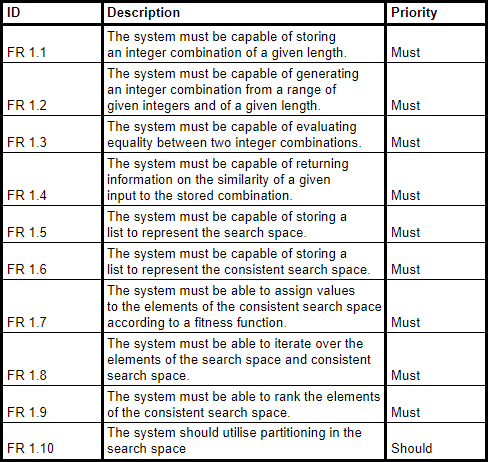
\includegraphics[scale=1]{Requirements}
\end{figure}

\newpage                     % optional page break
\section{Evaluation Strategy}\label{ss:back}

A solution for Mastermind can be defined as an algorithm that is able to consistently select the correct combination from a set of all possible combinations bounded by two parameters, the length of the combinations and the total number of symbols that a combination can be constructed from. This is the definition which is used to derive the metrics and methods by which the solution will be evaluated.

\subsection {Defining Metrics}

The following three metrics are used for evaluating a solution.
\begin {itemize}
	\item {The average number of guesses for the algorithm to arrive at the correct solution.}
	\item {The quantity of combinations reduced from the search space after each guess.}
	\item {The probability of selecting the correct combination from a set of conistent combinations \cite {ExhaustiveMM}.}
\end{itemize}

An additional argument can be made for measuring the time taken for an algorithm to terminate at the correct combination however this is dependent on the environment in which the algorithm is being hosted. The above metrics were chosen as they can be used to compare different algorithms accurately separate from the hosting environment

\newpage                     % optional page break
\section{Project Management}\label{ss:back}

\subsection {Gantt Chart}

The organisation of this project is represented by the following Gantt Chart, by utilising this chart the progress of later stages can be tracked and adjusted if there is a risk to the schedule.

\

\begin{figure}[H]
\centering
\caption[Short Heading]{Gantt Chart Organisation for Project.}
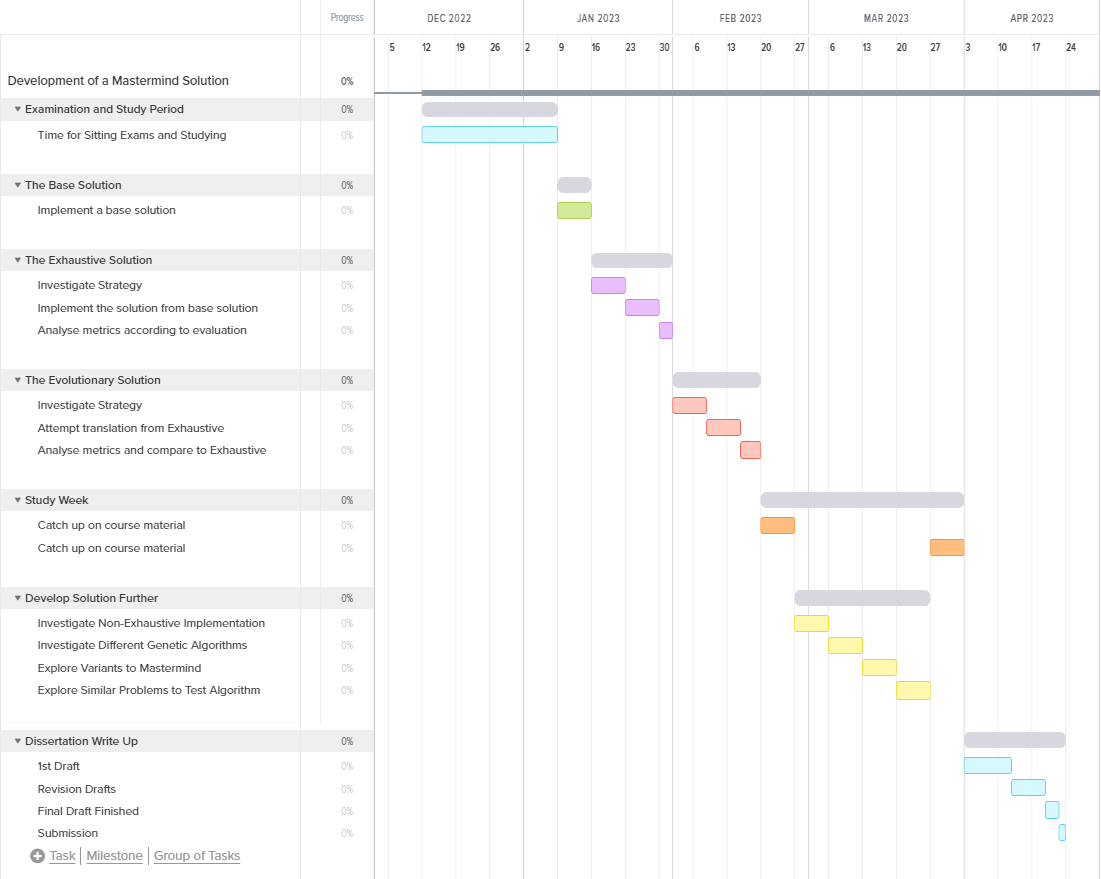
\includegraphics[scale=0.5]{Gantt}
\end{figure}

\

\subsection {Risk Analysis and Mitigations}

\subsubsection {Risk Definitions}
To manage the progress of this project efficiently it was important to identify possible risks that could prevent the realisation of the goals laid out earlier in this document. To aid in the identification of the risks the following key was used to classify the associated risks:
\begin{itemize}
\item{People (P) - Risks which are the result of issues related to those individuals involved in the project. This relates to the wellbeing, scheduling and personal issues that can be encountered.}
\item{Technological (T) - Risks which can result from the technology being used to engineer the solutions. This relates to the technological constraints that could be encountered or the hardware required.}
\item{Requirement (R)  - Risks which can result from changes to the requirements of the project. This relates to problems encountered with the work being implemented for the project. Logical problems and issues with the material involved would be included in these risks.}
\end{itemize}

\begin{figure}[H]
\centering
\caption[Short Heading]{Classification of Risks.}
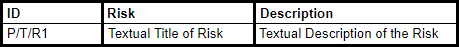
\includegraphics[scale=1]{RiskIdentify}
\end{figure}

\subsubsection {Risk Identification}

\begin{figure}[H]
\centering
\caption[Short Heading]{Identified Project Risks.}
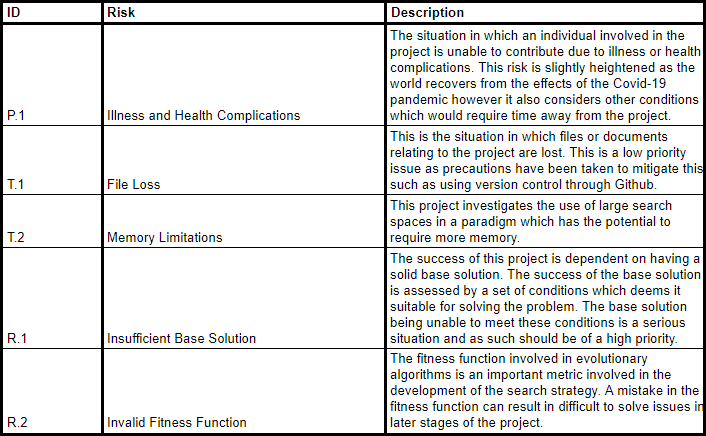
\includegraphics[scale=0.75]{Risks}
\end{figure}

\subsubsection {Risk Mitigation Procedures}

P.1:	Space has been allocated in the project timetable and schedule to allow for leniency in the  event of illness. If serious illness is encountered the University mitigating circumstances guidelines are available as an additional procedure.

T.2:	All contributions are stored remotely in a backup online repository.

T.2:	The scope of this project allows for the range of search spaces to remain within a feasible limit while still maintaining the ability to gather meaningful results.

R.1: 	Time in the schedule for the project has been allocated to prevent the effect that setbacks in the project can have. Any problems with solutions can serve as commentary to the implementation procedure.

R.2:	Fitness function security is to be closely monitored and testing procedures implemented to minimise the effects of an invalid fitness function in later stages.

\subsection {Considerations of Professional, Legal, Ethical, and Social Issues}

Professional consideration regarding this project extends to citations of work which has contributed to the contents of this investigation. It is important that any work which was not conducted by an individual involved in this project is correctly cited to avoid plagiarism.
Development software involved in this project should be legally obtained and operated.
This project does not involve any human subjects or the management of sensitive personal information which would require ethical or social consideration.




%%%%%%%%%%%%%%%%%%%%%%%%%%%%%%%%%%%%%%%%%
%
%     Bibliography
%
%     Use an easy-to-remember tag for each entry - eg \bibitem{How97} for an article/book by Howie in 1997
%     To cite this publication in your text, write \cite{How97}.  To include more details such as
%     page, Chapter, Theorem numbers, use the form \cite[Theorem 6.3, page 42]{How97}.
%
\begin{thebibliography}{99}

% 
% The usual convention for mathematical bibliographies is to list alphabetically
% by first-named author (then second, third  etc. author then date)
% websites with no author names should go by the site name
%

% Typical layout for reference to a journal article
%\bibitem{Bovey}
%J. D. Bovey, M. M. Dodson,                         % author(s)
%The Hausdorff dimension of systems of linear forms % article name
%{\em Acta Arithmetica}                             % journal name - italics
%{\bf 45}                                           % volume number - bold
%(1986), 337--358.                                   % (year), page range


% Typical layout for reference to a book
%
%\bibitem{Cassels}
%J. W. S. Cassels,                                  % author(s)
%{\em An Introduction to Diophantine Approximation},% title - italics
%Cambridge University Press, Cambridge, 1965.       % Publisher, place, date.

% Typical layout for reference to a website
%
%\bibitem{GAP}
%The GAP Group, GAP -- Groups, Algorithms, and Programming,  % Site name
%Version 4.5.6; 2012. % other information
%(http://www.gap-system.org)  % URL


% Typical layout for reference to an online article

%\bibitem{Howie}
%J. Howie,                                            % author(s)
%{\em Generalised triangle groups of type $(3,5,2)$}, % article name - italics
%http://arxiv.org/abs/1102.2073                       % URL
%(2011).                                              % (year)

\bibitem {Wordle}
New York Times,
{\em "Wordle".}
https://www.nytimes.com/games/wordle/index.html
(Online, accessed 21-11-2022)

\bibitem {Wolfram}
Weisstein, Eric W.
{\em '"Mastermind." From Mathworld -- A Wolfram Web Resource'.}
https://mathworld.wolfram.com/Mastermind.html
(Online; accessed \today)

\bibitem {Invicta}
Invicta Toys and Games ltd.
{\em 'History of Mastermind.'}
https://web.archive.org/web/20070812104420/http://dspace.dial.pipex.com/town/road/gbd76/toys.htm
(Archived 2007)

\bibitem {Better Solutions}
J.-J. Merelo and T. P. Runarsson,
Finding Better Solutions to the Mastermind Puzzle Using Evolutionary Algorithms.
{\em 'Applications of Evolutionary Computing'.}
{\bf vol 6024}
(2010), pp 121-130

\bibitem {SuperMM}
Noble Knight Games,
{\em 'Super Master Mind - Boardgame from Invicta Games'.}
https://www.nobleknight.com/P/2147590038/Super-MasterMind
(Online; accessed \today)

\bibitem {ExhaustiveMM}
Merelo, J.J., Mora, A.M., Cotta, C. and Runarsson, T.P. 
{\em  ‘An experimental study of exhaustive solutions for the Mastermind puzzle'.}
(2012)
 doi:10.48550/arxiv.1207.1315.

\bibitem {Nelson}
Nelson, Toby.
{\em 'Investigations into the MasterMind Board Game'.}
https://web.archive.org/web/20150906043015/http://www.tnelson.demon.co.uk/mastermind/index.html
(1999, Archived 2015)

\bibitem {Haystack}
Merelo-Guervós, J.J., Castillo, P. and Rivas, V.M. 
{\em ‘Finding a needle in a haystack using hints and evolutionary computation: the case of evolutionary MasterMind’, Applied soft computing}
{\bf  6(2)}
(2006) pp. 170–179. 
doi:10.1016/j.asoc.2004.09.003.

\bibitem {Two Peg}
Jäger, G.
An Optimal Strategy for Static Black-Peg Mastermind with Two Pegs.
{\em 'Combinatorial Optimization and Applications'.}
{\bf vol 10043}
(2016), pp 670–682
https://doi.org/10.1007/978-3-319-48749-6\_48

\bibitem {Knuth}
Knuth, Donald E. 
{\em 'The Computer as Master Mind', Recreational Mathematics}
{\bf 9(1)}
Stanford University
(1976, Baywood Publishing Co., Inc.)

\bibitem {Merelo}
 Merelo, J.J., Mora, A.M., Cotta, C. and Runarsson, T.P. 
{\em ‘An experimental study of exhaustive solutions for the Mastermind puzzle’.}
(2012) 

\bibitem {ExhaustiveDef}
Weisstein, Eric W.
{\em '"Exhaustive Search." From Mathworld -- A Wolfram Web Resource'.}
https://mathworld.wolfram.com/ExhaustiveSearch.html
(Online; accessed \today)

\bibitem {MMNP}
Stuckman, J. and Zhang, G.-Q.
{\em  ‘Mastermind is NP-Complete’.}
(2005)
doi:10.48550/arxiv.cs/0512049.

\bibitem {NP}
Weisstein, Eric W.
{\em 'NP-Problem' From Mathworld -- A Wolfram Web Resource'.}
https://mathworld.wolfram.com/NP-Problem.html
(Online; accessed \today)

\bibitem {Yet}
Kooi, B.
‘Yet another mastermind strategy’,
{\em ICGA Journal}
{\bf 28(1)}
pp. 13-20.

\bibitem {Evo}
P. A. Vikhar,
'Evolutionary algorithms: A critical review and its future prospects',
{\em International Conference on Global Trends in Signal Processing, Information Computing and Communication (ICGTSPICC)}
(2016)
pp. 261-265
doi: 10.1109/ICGTSPICC.2016.7955308

\bibitem {RSA}
Abualigah, L., Elaziz, M.A., Sumari, P., Geem, Z.W. and Gandomi, A.H. 
‘Reptile Search Algorithm (RSA): A nature-inspired meta-heuristic optimizer’,
{\em  Expert systems with applications}
{\bf 191}
(2022), 
pp. 116-158.
 doi:10.1016/j.eswa.2021.116158.

\bibitem {Practical Haskell}
Serrano Mena, A. 
{\em 'Practical Haskell'.}
(2022) Berkeley, CA: 
Apress L. P.

\bibitem {Functional Genetics}
Briggs, Forrest., O'Neill, Melissa. 
'Functional Genetic Programming and Exhaustive Program Search with Combinator Expressions'.
{\em International Journal of Knowledge-based and Intelligent Engineering Systems.}
{\bf 12}
(2008),
pp 47-68. 
10.3233/KES-2008-12105. 

\bibitem {Pearls}
Bird, Richard.
{\em How to Write a Functional Pearl}
International Conference on Functional Programming, Portland
(2006)

\bibitem {R. Bird Speech}
Gibbons, Jeremy.
{\em University of Oxford, Functional Pearls}
http://www.cs.ox.ac.uk/people/jeremy.gibbons/pearls/
(2009)

\bibitem {Sudoku}
Bird, Richard.
{\em Functional Pearl, A Program to Solve Sudoku}
Cambridge University Press, Cambridge, 2006

\end{thebibliography}
\end{document}
